\chapter{Applications}
\label{chap:applications}

In this chapter, we apply the models developed earlier to two selected problems. The first problem is the Lotka-Volterra model described in \autoref{sec:lotka-volterra}, the second is a simple model for auto-regulation in prokaryotes considered in \autoref{sec:autoregulation}. The particle filter-based approach is compared with the one depending on ABC methods in various settings and model misspecifications.

Both problems require simulating reactions in order to propagate the system states through time. This is done with the help of the Gillespie algorithm, which is first described in \autoref{sec:gillespie}.

\section{Preliminary: the Gillespie algorithm} \label{sec:gillespie}
The Gillespie algorithm \citep{gillespie1, gillespie2} is used to simulate a stochastic process describing the time evolution of a system of reactions. The discussion given here follows \cite{wilkinson-book}.

\paragraph{Time evolution of a reaction system}
Consider a system consisting of $u$ species $\mathcal{X}_1, \ldots, \mathcal{X}_u$ and $v$ reactions $\mathcal{R}_1, \ldots, \mathcal{R}_v$. The species can describe literal animal species, as is the case in the Lotka-Volterra model in \autoref{sec:lotka-volterra}, or individual molecule types, as in \autoref{sec:autoregulation}. The reactions describe the interactions between these species through time.

Let the number of molecules (or individuals, in case of animal species) of the species $\mathcal{X}_i$ at time $t$ be denoted by $X_{i,t}$, and let $\bm{X}_t = \left(X_{1,t}, \ldots, X_{u,t}\right)^\intercal$. Additionally, let the number of reactions of type $\mathcal{R}_i$ which occurred in a time window $(0, t]$ be denoted by $R_{i,t}$, and let $\bm{R}_t = \left(R_{1,t}, \ldots,R_{v,t}\right)^\intercal$. The evolution of the system from time 0 to time $t$ is described by the equation
\begin{equation} \label{eq:system-evolution}
\bm{X}_t - \bm{X}_0 = \mathbb{S}\bm{R}_t,
\end{equation}
where $\mathbb{S} \in \R^{u \times v}$ is called the stoichiometry matrix of the system, and describes the difference in the number of molecules of each species after each reaction occurs. To gain insight into the meaning of $\mathbb{S}$, it is instructive to write it as
\begin{equation*}
\mathbb{S} = \mathbb{P}_\text{post} - \mathbb{P}_\text{pre},
\end{equation*}
where the element $(i,j)$ of $\mathbb{P}_\text{pre}$ denotes the number of molecules of $\mathcal{X}_i$ before a reaction of type $\mathcal{R}_j$ takes place, and the element $(i,j)$ of $\mathbb{P}_\text{post}$ describes the same quantity \emph{after} it takes place. Equation \eqref{eq:system-evolution} can then be written as
\begin{equation*}
\bm{X}_t = \bm{X}_0 + \left(\mathbb{P}_\text{post} - \mathbb{P}_\text{pre}\right) \bm{R}_t,
\end{equation*}
and describes the net gain in the number of molecules of each species, given their initial numbers, and accounting for their increase/decrease when a number of reactions of each type occurs.

In addition, each reaction $\mathcal{R}_i$ has a stochastic rate constant $c_i$ and a rate law (also called the hazard function) $h_i(\bm{X}_t, c_i)$ associated with it. The interpretation of the hazard function is such that $h_i(\bm{X}_t, c_i) \dx{t}$ is the probability of a reaction of type $\mathcal{R}_i$ occurring in a time interval $(t, t + \dx{t}]$, conditionally on the system being in state $\bm{X}_t$. Such a situation is described by an exponential distribution -- the time to the event of a reaction of type $\mathcal{R}_i$ occurring, assuming no other reaction is taking place, is distributed according to ${\mathcal{E}\mathit{xp}\left(h_i(\bm{X}_t, c_i)\right)}$. This is however a convenient simplification, since multiple reactions are typically occurring at the same time.

\paragraph{The Gillespie algorithm}
In a system with $v$ reactions and their hazard functions $h_i(\bm{X}_t, c_i)$, the hazard of \emph{some} reaction occurring is
\begin{equation*}
h_0(\bm{X}_t, \bm{c}) = \sum_{i=0}^v h_i(\bm{X}_t, c_i),
\end{equation*}
where $\bm{c} = \left(c_1, \ldots, c_v\right)^\intercal$. The time to the next reaction is then distributed according to $\mathcal{E}\mathit{xp}\left(h_0(\bm{X}_t, \bm{c})\right)$. The particular reaction type is a random variable with a categorical distribution $\mathcal{C}\mathit{at}\left(\widetilde{h}_1(\bm{X}_t,c_1), \ldots, \widetilde{h}_v(\bm{X}_t,c_v)\right)$, where $\displaystyle \widetilde{h}_i(\bm{X}_t,c_i) = \frac{h_i(\bm{X}_t,c_i)}{h_0(\bm{X}_t, \bm{c})}$.

With the above in mind, the Gillespie algorithm can now be formulated, and is given in \autoref{alg:gillespie}. Its purpose is to simulate the state evolution \eqref{eq:system-evolution} for a given time horizon $T$ while accounting for the randomness in the time until a reaction of a particular type takes place. For the purpose of this algorithm, denote the columns of the stoichiometry matrix $\mathbb{S}$ by $\bm{S}^i, \quad i = 1, \ldots, v$.
\begin{algorithm}[ht]
    \caption{Gillespie algorithm}
    \label{alg:gillespie}
    \begin{algorithmic}[1]
        \Input $\text{Time horizon } T, \text{ rate constants } \bm{c} = \left(c_1, \ldots, c_v\right)^\intercal,\ \text{initial molecule numbers } \bm{X}_0.$
        
        \State $t \gets 0$
        
        \State $\bm{X}_t \gets \bm{X}_0$
        
        \While{$t \leq T$}
            \State $\text{Calculate } h_i(\bm{X}_t, c_i), \quad i = 1, \ldots, v.$
            \State $h_0(\bm{X}_t, \bm{c}) \gets \sum_{i=1}^v h_i(\bm{X}_t, c_i)$
            \State $\text{Calculate } \displaystyle \widetilde{h}_i(\bm{X}_t,c_i) = \frac{h_i(\bm{X}_t,c_i)}{h_0(\bm{X}_t, \bm{c})}, \quad i = 1, \ldots, v.$
            \State $\text{Sample } \dx{t} \sim \mathcal{E}\mathit{xp}\left(h_0(\bm{X}_t, \bm{c})\right).$ \Comment{Simulate the time to the next reaction.}
            \State $\text{Sample } i \sim \mathcal{C}\mathit{at}\left(\widetilde{h}_1(\bm{X}_t,c_1), \ldots, \widetilde{h}_v(\bm{X}_t,c_v)\right).$ \Comment{Simulate the reaction type.}
            \State $\bm{X}_{t + \dx{t}} \gets \bm{X}_t + \bm{S}^i$ \Comment{Update the state according to the reaction $i$.}
            \State $t \gets t + \dx{t}$
        \EndWhile
        
        \Output $\text{Final state } \bm{X}_t, \text { final time } t.$
    \end{algorithmic}
\end{algorithm}

The algorithm is usually the bottleneck of most simulations, and must be implemented carefully; otherwise, the simulation becomes unacceptably slow. The final time $t$ is at the output as well, since it may exceed the horizon $T$. If the algorithm is run consecutively during a simulation, the interest is to follow the previous run by starting at its final time $t$.

\section{Lotka-Volterra model} \label{sec:lotka-volterra}
\subsection{Problem description}
The first considered problem is the Lotka-Volterra model \citep{lotka, volterra}. The system describes a simplified time interaction of a population consisting of a predator and prey species. Denoting the prey species by $\mathcal{X}_1$ and the predator species by $\mathcal{X}_2$, the system can be described by the reactions
\begin{align}
\mathcal{R}_1:\quad & \mathcal{X}_1 \to 2 \mathcal{X}_1, \label{eq:lv1} \\
\mathcal{R}_2:\quad & \mathcal{X}_1 + \mathcal{X}_2 \to 2 \mathcal{X}_2, \label{eq:lv2} \\
\mathcal{R}_3:\quad & \mathcal{X}_2 \to \emptyset. \label{eq:lv3}
\end{align}
Equation \eqref{eq:lv1} describes the reproduction of the prey species. Equation \eqref{eq:lv2} describes the interaction between the predator and the prey where a predator consumes an individual of the prey species and produces an offspring. Equation \eqref{eq:lv3} describes the extinction of the predator species when no prey is present.

The state of the system at time $t$ is $\bm{X}_t = \left(X_{1,t}, X_{2,t}\right)^\intercal$. The stoichiometry matrix is given by
\begin{equation*}
\mathbb{S} = \begin{pmatrix}
1 & -1 & 0 \\
0 & 1 & -1 \\
\end{pmatrix},
\end{equation*}
and the hazard functions vector is $\bm{h}(\bm{X}_t, \bm{c}) = \left(c_1 X_{1,t}, c_2 X_{1,t} X_{2,t}, c_3 X_{2,t}\right)^\intercal$ \citep{wilkinson}. Although simple to describe, this model is analytically intractable \citep{wilkinson-book}.

For the inference problem, we consider the unknown parameters to be $\btheta = \left(c_1, c_2, c_3\right)^\intercal$, and the state at time $t$ to be $\bx_t = \left(X_{1,t}, X_{2,t}\right)$. Since the rate constants $c_1, c_2, c_3$ are by definition positive, we are working in the log space to avoid restricting ourselves to positive support distributions. The model is specified by the following:
\begin{equation*}
\begin{split}
\sprior(x_{1,0} \mid \btheta) &= \mathcal{P}\mathit{o}\left(50\right), \\
\sprior(x_{2,0} \mid \btheta) &= \mathcal{P}\mathit{o}\left(100\right), \\
\trans_t(\bx_t \mid \bx_{t-1}, \btheta) & \text{ is simulated using \autoref{alg:gillespie} }, \\
\obs_t(\by_t \mid \bx_{t}, \btheta) &= \mathcal{N}_2\left(\bx_t, 10^2\right).
\end{split}
\end{equation*}
The parameter prior and the Metropolis-Hastings proposal are additionally given by
\begin{equation*}
\begin{split}
\pprior(\log c_i) &= \mathcal{U}\left(-7, 2\right), \quad i = 1, 2, 3, \\
\prop(\btheta^\prime \mid \btheta) &= \mathcal{N}_3\left(\btheta, \text{diag}\left(0.01, 0.01, 0.01\right)\right).
\end{split}
\end{equation*}
The initial parameters are $\btheta^{(0)} = \left(1, 0.005, 0.6\right)^\intercal$. We are working with a dataset simulated using \autoref{alg:gillespie} ran so that it outputs 16 observations $\by_t$, starting from the same parameters $\btheta^{(0)}$. The inference is started in the correct parameters and applied on a short sequence only; its purpose is only to demonstrate that the algorithm is able to identify these parameters.

We apply the marginal Metropolis-Hastings algorithm depending on the particle filter as well as the one utilizing ABC methods. Both algorithms are ran for $M = 50000$ samples with $N = 100$ particles. Additionally, the number of covered pseudo-observations in the ABC formulation is $\alpha = 95$ and the volume of the p-HPR is $p = 0.95$.

\subsection{Inference using the particle filter}
In this section, we consider inference using \autoref{alg:marginal-metropolis-hastings}, i.e. using the particle filter to approximate the likelihood.

\paragraph{Correctly specified observation model}
At first, we assume the correct model specification. This means that the observations $\by_t$ have been corrupted by Gaussian noise, and the observation model $\obs_t$ is Gaussian as well. In this situation, the particle filter is expected to perform well, as all assumptions have been met.

In \autoref{fig:lv-pmh-gauss-c1}, \autoref{fig:lv-pmh-gauss-c2} and \autoref{fig:lv-pmh-gauss-c3}, the results for the parameters $c_1$, $c_2$ and $c_3$, respectively, are shown. For each parameter, we show (in this order) the trace plot, the autocorrelation plot, and the histogram of sampled values. We use no burn-in period, as the inference starts in the correct values, but apply thinning of 100, i.e. keep every 100th sample. This ensures relatively uncorrelated samples, as is clear from the auto-correlation plots. The acceptation rate of the Metropolis-Hastings algorithms moves around 20 \%.

\begin{figure}[ht]
    \centering
    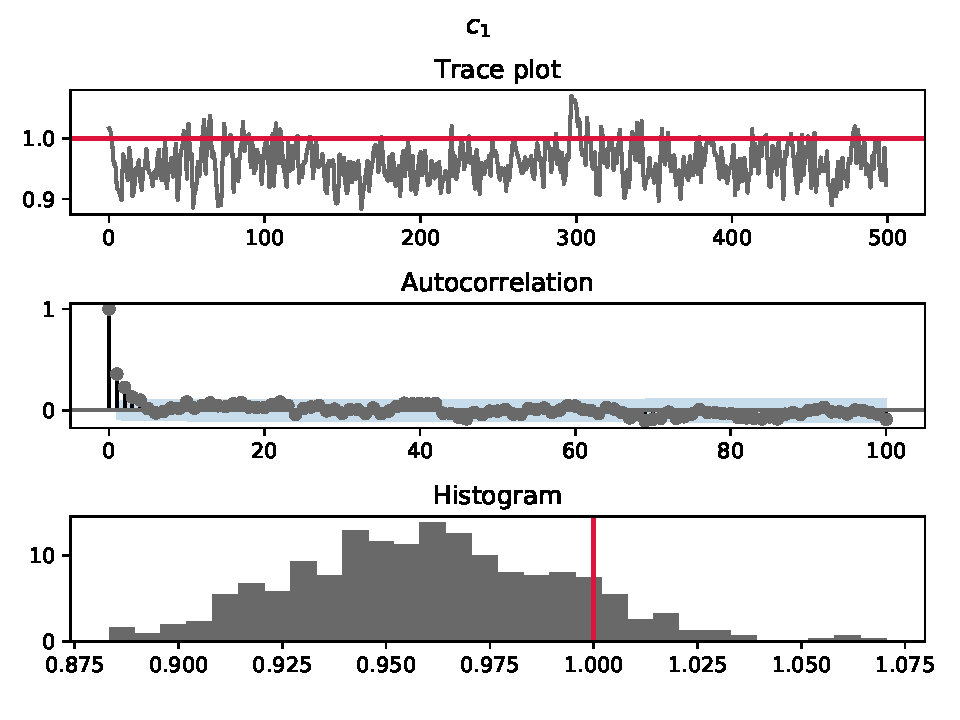
\includegraphics[width=0.7\linewidth]{lotka-volterra/pmh_gauss_c1}
    \caption{Particle filter-based inference of the parameter $c_1$ in the Lotka-Volterra model. Uses Gaussian noise and a Gaussian observation model. The true value is shown in red.}
    \label{fig:lv-pmh-gauss-c1}
\end{figure}

\begin{figure}[ht]
    \centering
    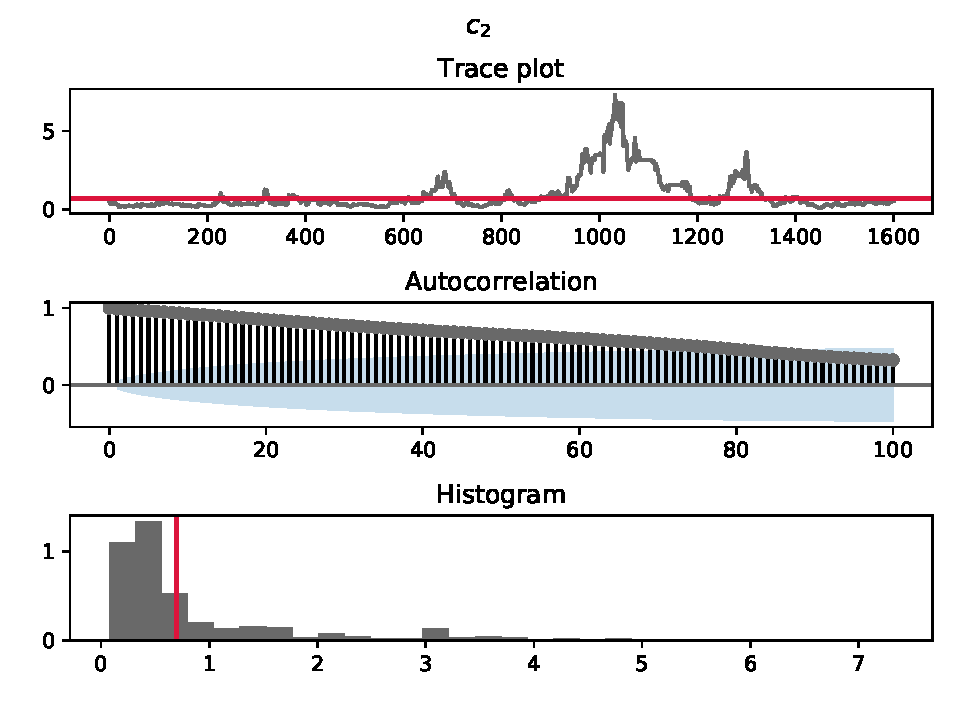
\includegraphics[width=0.7\linewidth]{lotka-volterra/pmh_gauss_c2}
    \caption{Particle filter-based inference of the parameter $c_2$ in the Lotka-Volterra model. Uses Gaussian noise and a Gaussian observation model. The true value is shown in red.}
    \label{fig:lv-pmh-gauss-c2}
\end{figure}

\begin{figure}[ht]
    \centering
    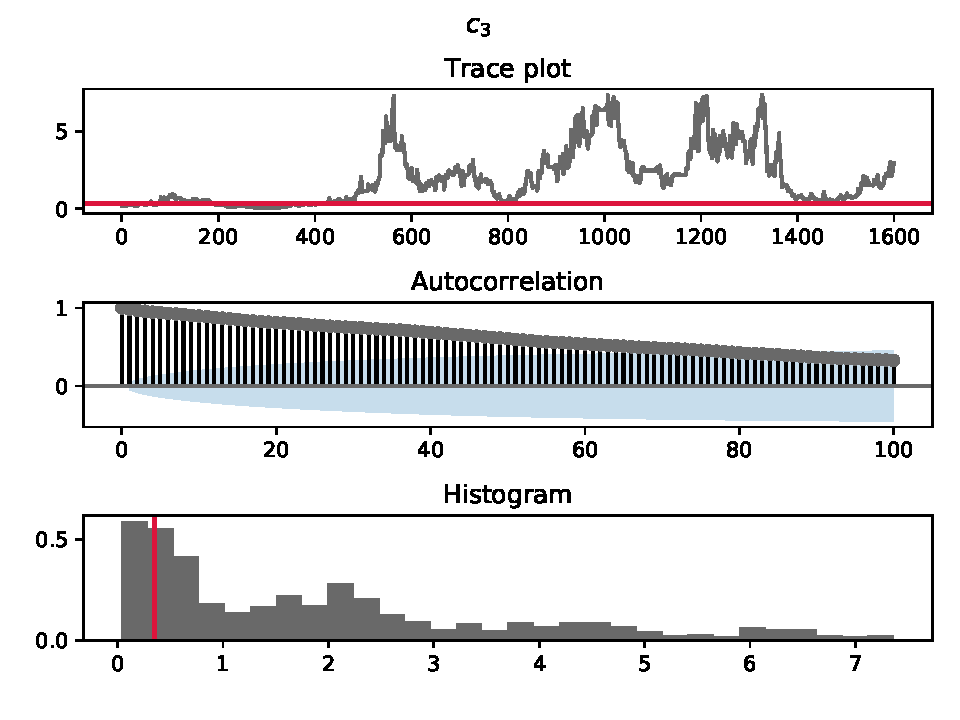
\includegraphics[width=0.7\linewidth]{lotka-volterra/pmh_gauss_c3}
    \caption{Particle filter-based inference of the parameter $c_3$ in the Lotka-Volterra model. Uses Gaussian noise and a Gaussian observation model. The true value is shown in red.}
    \label{fig:lv-pmh-gauss-c3}
\end{figure}

In all cases, the correct parameters are well-covered by the sampled values, while allowing for some degree of variance. The histograms provide estimated posterior distributions of the individual parameters. The sampled values can be used to provide point estimates or credible intervals for the true parameters.

\paragraph{Misspecified observation model}
Next, we keep the Gaussian observation model, but corrupt the observation sequence by a Cauchy noise with scale 10. Arguably, this scale is quite high, but is used to match the scale of the Gaussian noise from the previous section. The heavy-tailed Cauchy distribution allows sampling distant noise terms, and corrupts the observation sequence $\by_t$ much more severely. The Gaussian observation model $\obs_t$ then assigns probability close to zero to these values, and the filter collapses. This is clear from \autoref{fig:lv-pmh-cauchy-c1}, \autoref{fig:lv-pmh-cauchy-c2} and \autoref{fig:lv-pmh-cauchy-c3}.

\begin{figure}[ht]
    \centering
    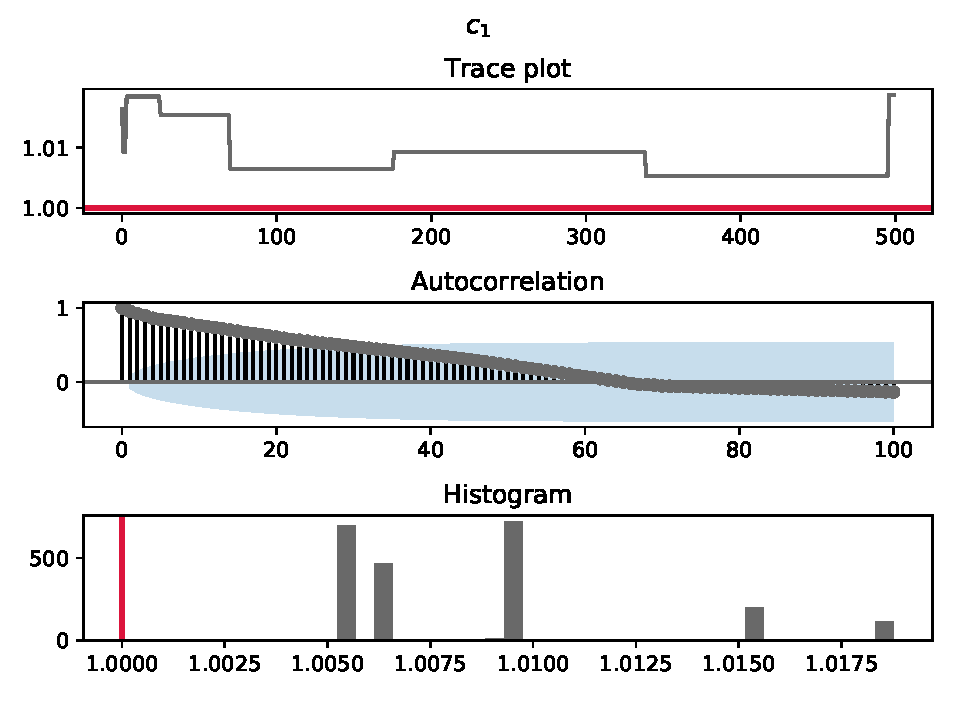
\includegraphics[width=0.7\linewidth]{lotka-volterra/pmh_cauchy_c1}
    \caption{Particle filter-based inference of the parameter $c_1$ in the Lotka-Volterra model. Uses Cauchy noise and a Gaussian observation model. The true value is shown in red.}
    \label{fig:lv-pmh-cauchy-c1}
\end{figure}

\begin{figure}[ht]
    \centering
    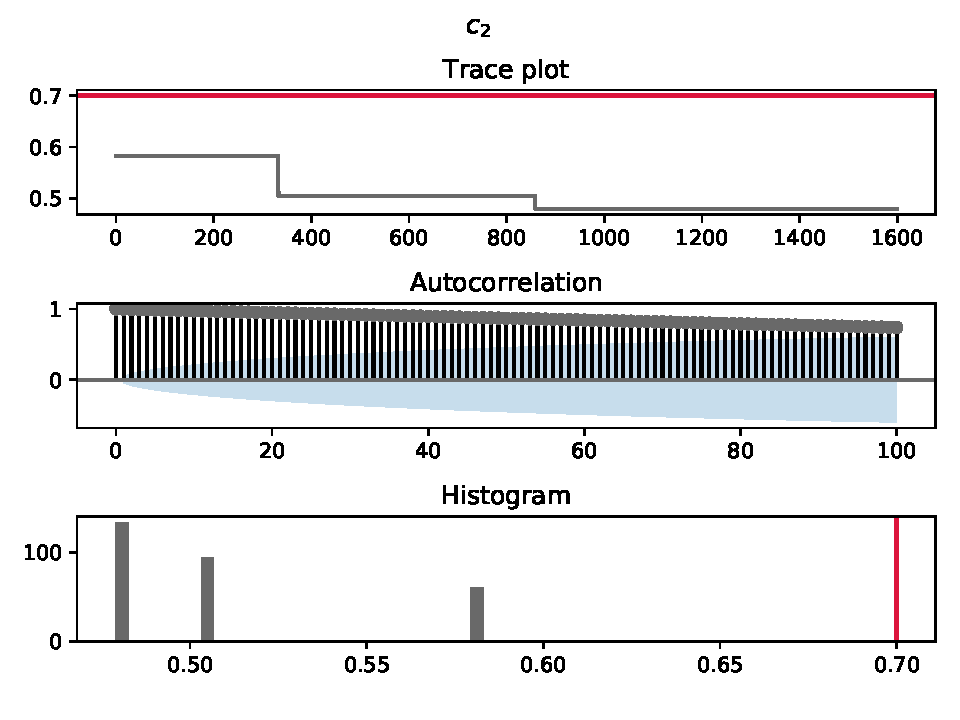
\includegraphics[width=0.7\linewidth]{lotka-volterra/pmh_cauchy_c2}
    \caption{Particle filter-based inference of the parameter $c_2$ in the Lotka-Volterra model. Uses Cauchy noise and a Gaussian observation model. The true value is shown in red.}
    \label{fig:lv-pmh-cauchy-c2}
\end{figure}

\begin{figure}[ht]
    \centering
    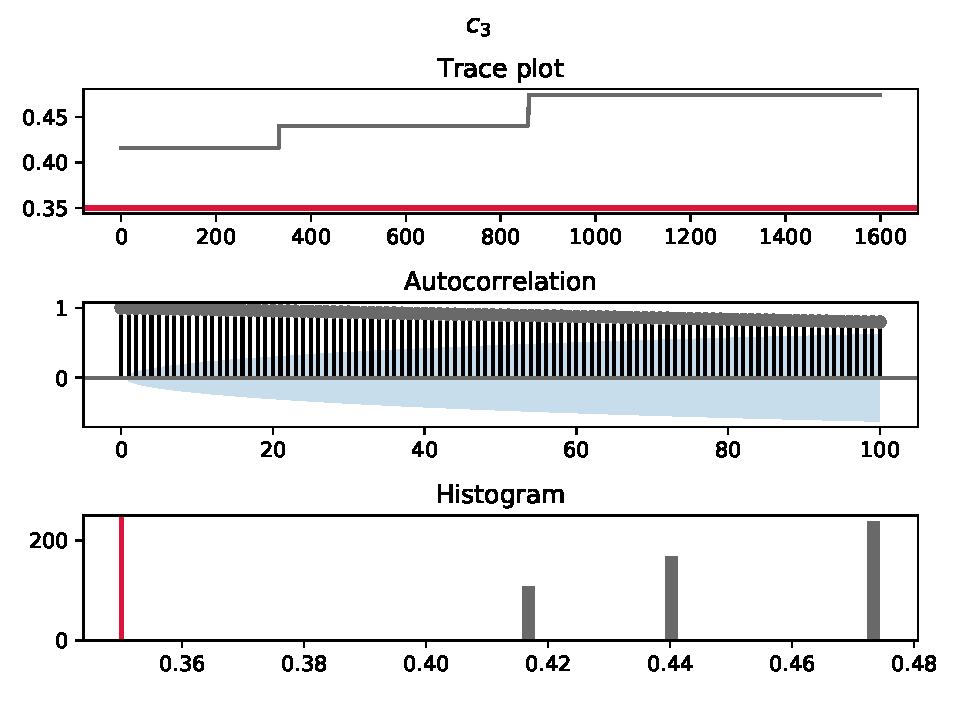
\includegraphics[width=0.7\linewidth]{lotka-volterra/pmh_cauchy_c3}
    \caption{Particle filter-based inference of the parameter $c_3$ in the Lotka-Volterra model. Uses Cauchy noise and a Gaussian observation model. The true value is shown in red.}
    \label{fig:lv-pmh-cauchy-c3}
\end{figure}

Clearly, Cauchy noise corrupts the sequence too much, and the results are miserable. The accepted parameters are almost constant, and the posterior distribution is not even remotely-well approximated. This is an expected behavior, since the particle filter is known not to perform well under model misspecification.



\subsection{Inference using ABC}
In this section, we apply \autoref{alg:marginal-metropolis-hastings-abc}, the variant of the Metropolis-Hastings algorithm depending on ABC.



\section{Prokaryotic auto-regulation model} \label{sec:autoregulation}
\subsection{Problem description}

\subsection{Inference using the particle filter}

\subsection{Inference using ABC}